\begin{figure}[htbp]
\centering
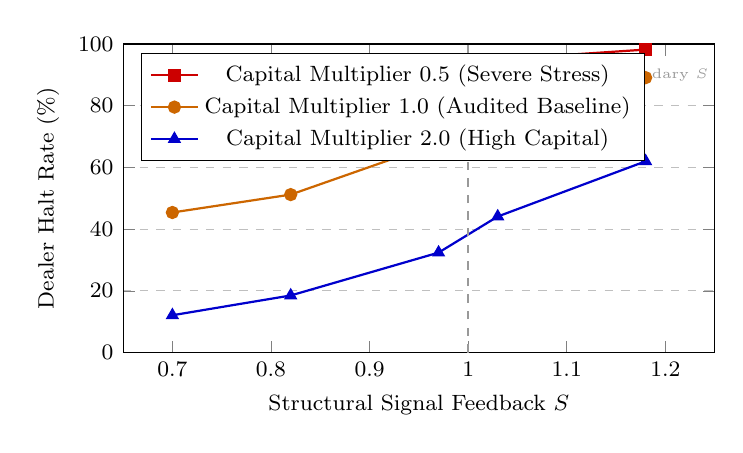
\begin{tikzpicture}
\begin{axis}[
    width=0.75\textwidth,
    height=5.5cm,
    xlabel={Structural Signal Feedback $S$},
    ylabel={Dealer Halt Rate (\%)},
    xmin=0.65, xmax=1.25,
    ymin=0, ymax=100,
    legend pos=north west,
    ymajorgrids=true,
    grid style=dashed,
    font=\footnotesize
]
\addplot[color=red!80!black, mark=square*, thick] coordinates {
    (0.70, 85.2) (0.82, 88.4) (0.97, 92.1) (1.03, 95.0) (1.18, 98.2)
};
\addlegendentry{Capital Multiplier 0.5 (Severe Stress)}

\addplot[color=orange!80!black, mark=*, thick] coordinates {
    (0.70, 45.4) (0.82, 51.2) (0.97, 68.0) (1.03, 76.5) (1.18, 89.1)
};
\addlegendentry{Capital Multiplier 1.0 (Audited Baseline)}

\addplot[color=blue!80!black, mark=triangle*, thick] coordinates {
    (0.70, 12.1) (0.82, 18.5) (0.97, 32.4) (1.03, 44.1) (1.18, 62.0)
};
\addlegendentry{Capital Multiplier 2.0 (High Capital)}

\draw[thick, black!40, dashed] (axis cs:1.0, 0) -- (axis cs:1.0, 100)
    node[pos=0.9, right, font=\tiny]{Signal stability boundary $S=1$};
\end{axis}
\end{tikzpicture}
\caption{Decoupling of signal feedback $S$ from operational dealer halt rates across balance-sheet capital multipliers under repricing shock $\mu = -2.0$.}
\label{fig:F5_signal_vs_funded_risk}
\end{figure}
